\documentclass[a4paper, 12pt]{report}
\pagestyle{headings}

\usepackage{graphicx}
\graphicspath{ {image/} }

\usepackage{calc}
\usepackage{enumitem}
\usepackage{nameref}

\newenvironment{mydescription}[1]
  {\begin{list}{}%
   {\renewcommand\makelabel[1]{##1:\hfill}%
   \settowidth\labelwidth{\makelabel{#1}}%
   \setlength\leftmargin{\labelwidth}
   \addtolength\leftmargin{\labelsep}}}
  {\end{list}}

%\renewcommand{\descriptionlabel}[1]{\hspace{1cm}\textsf{#1}\hfill}

\begin{document}

\title{File System}
\author{Ricky Hariady}

\maketitle

\chapter{Gambaran Umum}
\label{overview}

Bagian ini menjelaskan secara umum mengenai \emph{file system} yang akan digunakan pada \emph{pintarOS}. Sebagaimana dapat dilihat pada rancangan utama, \emph{file system} berfungsi menangani struktur file dan operasi-operasi yang dapat dilakukan terhadap file tersebut. Bagaimana data file tersebut disimpan pada memory fisik tidak menjadi tanggung jawab File System karena akan dilakukan oleh \emph{HAL Memory} dengan  menyediakan layanan untuk penyimpanan dan pengambilan data dari Non-Volatile Memory (NVM) menggunakan pengalamatan yang linier dan kontinyu.

\section{Struktur File System}
\label{file-system-structure}

Sebagaimana dijelaskan pada dokumen ISO 7816-4, terdapat dua jenis file dasar yang dapat digunakan pada \textsl{smart card} yaitu :
\begin{itemize}
\item Elementary File (EF), dan
\item Dedicated File (DF).
\end{itemize}

\emph{Elementary File} merupakan jenis file yang dapat menyimpan data aktual. Sedangkan \emph{dedicated File} merupakan file khusus yang tidak berfungsi menyimpan data aktual, melainkan memuat daftar sejumlah file lainnya (dapat berupa EF maupun DF). Fungsi DF ini dapat disamakan dengan fungsi \emph{directory} pada komputer PC. Dengan mengelompokkan sejumlah file yang saling berkaitan dalam sebuah DF (sebagai contoh dalam sebuah aplikasi) akan menghasilkan sebuah sistem file yang terstruktur. Sejumlah file DF ini kemudian dapat dikelompokkan kembali dalam file DF lainnya dengan level yang lebih tinggi. Sebuah \emph{Dedicated File} khusus yang menempati lokasi tertinggi (\emph{root}) dalam struktur file system kemudian disebut sebagai \emph{Master File} (MF). Gambar \ref{fig-fs-example} menampilkan contoh struktur file system dari sebuah \textsl{smart card} yang terdiri dari sebuah MF serta sejumlah DF dan EF.

\begin{figure}
\centering
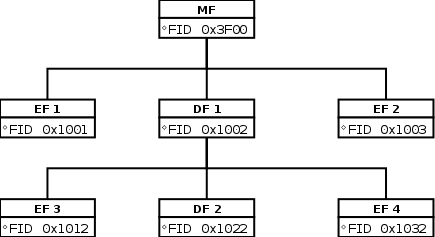
\includegraphics[width=0.7\textwidth]{fs_example.png}
\caption{struktur file system}
\label{fig-fs-example}
\end{figure}

\section{Atribut File}
\label{file-attribute}

Setiap file pada \textsl{smart card} dikenali melalui FID dari file tersebut. Untuk mencegah ambiguitas, maka file-file yang berada dalam 1 DF tidak boleh memiliki FID yang sama (demikian pula dengan DF induknya). 

Dilihat dari sisi penggunanya, \emph{Elementary File} (EF) dibagi menjadi dua jenis, yaitu :
\begin{itemize}
\item Working EF, dan 
\item Internal EF.
\end{itemize}

 \emph{Working} EF adalah EF yang menyimpan data-data milik aplikasi \textsl{smart card} dan dapat diakses oleh aplikasi. Sementara \emph{internal} EF adalah EF yang menyimpan data-data milik \emph{operating system} dan tidak dapat diakses langsung oleh aplikasi. Contoh \emph{internal} EF misalnya adalah file EF yang menyimpan kunci keamanan. Kunci yang disimpan dalam file ini akan dibaca oleh \emph{operating syste}m dan dicocokkan dengan kunci yang diberikan oleh pengguna \textsl{smart card} untuk memperoleh hak untuk mengakses file-file lainnya didalam DF.

Standar ISO 7816-4 memberikan 5 struktur internal berbeda yang mungkin digunakan pada sebuah file EF, yaitu :
\begin {itemize}
\item Transparent
\item Linier Record (fixed length)
\item Linier Record (variable length)
\item Cyclic Record
\item TLV
\end {itemize}

Selain jenis (\emph{working} atau \emph{internal}) dan struktur internalnya EF, terdapat sejumlah atribut lainnya yang dapat melekat pada sebuah file, diantaranya :
\begin {itemize}
\item read-write/read-only
\item shareable/not-shareable
\item access condition
\end {itemize}

\section{Operasi file}
\label{file-operation}

Sebagaimana pada sistem komputer lainnya, pengguna dapat melakukan sejumlah operasi terhadap file. Operasi-operasi file yang dapat dilakukan pada \textsl{smart card} mencakup:

\begin{itemize}
\item Menciptakan file
\item Menghapus file
\item Memilih file
\item Menulis file
\item Membaca file
\item Mengubah atribut file
\end{itemize}

\section{Keamanan file}
\label{file-security}

Salah satu faktor penting yang menjadi kelebihan \textsl{smart card} dibanding kartu elektronik lainnya adalah dari segi keamanan. Demikian pula terhadap file yang disimpan didalamnya (dalam hal ini oleh \emph{file system}). Untuk mencapai tingkat keamanan tersebut, pengguna harus terlebih dahulu memenuhi kondisi tertentu untuk dapat mengakses sebuah file. Kondisi yang diperlukan ini selanjutnya disebut juga sebagai \emph{Access Condition} (AC). Metode yang akan digunakan untuk mengimplementasikan \emph{access condition} ini adalah dengan menggunakan \emph{security state}. Pada metode ini, pengguna harus mencapai \emph{security state} tertentu (melalui verifikasi PIN) untuk dapat mengakses sebuah file. \emph{Security state} yang dibutuhkan dapat berbeda untuk setiap operasi, sehingga dibutuhkan sebuah access condition untuk setiap operasi. 

\begin{itemize}
\item access condition untuk membaca,
\item access condition untuk menulis,
\item access condition untuk menghapus file,
\item access condition untuk menciptakan file baru (khusus DF).
\item access condition untuk mengubah atribut
\end{itemize}

\chapter{Design}
\label{design}

Bagian ini menjelaskan struktur data dan algoritma yang akan digunakan pada \emph{file system}.

\section{Data Structure}
\label{data-structure}

\subsection{Konsep Block}
\label{block-concept}

Sebagaimana telah disebutkan pada \nameref{overview}, \emph{file system} menggunakan layanan dari \emph{HAL Memory} untuk mengakses data file pada memory fisik. \emph{HAL memory} menyediakan ruang penyimpanan virtual yang menggunakan  pengalamatan linier dan kontinyu dimana setiap alamat dapat menyimpan data sebesar 1 byte. Namun penggunaan alamat untuk setiap 1 byte data ini kurang efisien dari sisi \emph{file system} karena akan membutuhkan ruang yang besar untuk menyimpan alamat sebuah file. Sebagai contoh, untuk memory berukuran 128 kB sebagaimana banyak ditemukan pada \textsl{smart card} terbaru membutuhkan ruang untuk alamat sebanyak 3 byte (dengan asumsi unit penyimpanan terkecil 1 byte). Pada kenyataannya sebuah file umumnya juga memiliki ukuran yang jauh lebih besar. Maka, untuk meningkatkan efisiensi penggunaan ruang memory digunakan konsep \emph{block} sebagai unit terkecil untuk mengalamati sebuah file dari sisi \emph{file system}, dimana satu \emph{block}x terdiri dari beberapa \emph{byte} memory. Sebagai contoh, untuk ukuran \emph{block} sebesar 4 byte, \emph{block} \texttt{0} merujuk pada alamat \texttt{0x0000} hingga \texttt{0x0003}, \emph{block} \texttt{1} merujuk pada alamat \texttt{0x0004} hingga \texttt{0x0007}, dan demikian seterusnya. Secara umum, alamat yang dirujuk dari sebuah \emph{block} dapat diketahui menggunakan:
$$
address=block\_number \cdot block\_size
$$


\begin{figure}[h]
\centering
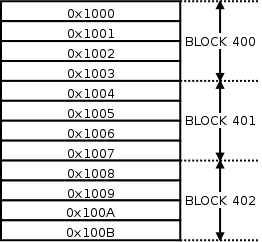
\includegraphics[width=0.5\textwidth]{fs_blocks.png}
\caption{Konsep Block}
\label{fig-block-concept}
\end{figure}

Konsep {\em block} ini mengadopsi {\em file system} pada PC seperti Unix File System ataupun FAT. Namun berbeda dengan {\em file system} tersebut dimana block juga menjadi unit operasi terkecil yang dapat dilakukan, pada {\em file system} yang dirancang, {\em block} hanya berfungsi sebagai unit pengalamatan terkecil. Operasi terhadap file tetap menggunakan unit {\em byte}. File system hanya akan membaca sejumlah {\em byte} yang diminta tidak perduli berapapun ukuran {\em block} yang digunakan. Demikian pula awal operasi pembacaan/penulisan dilakukan berdasarkan {\em offset} yang diukur dalam unit {\em byte}. Lebih jauh lagi penggunaan konsep {\em block} juga membantu dalam mengetahui bagian mana dari {\em virtual memory} yang telah digunakan (lebih lanjut akan dijelaskan pada \nameref{bat}).

Disamping kelebihannya, penggunaan konsep {\em block} juga memiliki kelemahan yaitu pemborosan yang terjadi apabila ternyata hanya sebagian dari {\em block} yang digunakan untuk menyimpan data. Kerugian ini menjadi lebih terasa apabila menggunakan ukuran {\em block} yang besar. Sebagaimana telah disebutkan {\em block} merupakan unit terkecil pengalamatan file, maka ketika sebuah file membutuhkan ruang sebesar 9 byte, dengan ukuran {\em block} sebesar 8 byte, akan menggunakan sebanyak {\tt 2} {\em block} (= 16 {\em byte}). Selisih sebesar 7 (=16-9) {\em byte} ini kemudian menjadi percuma karena tidak dapat digunakan. Pada sistem komputer PC kerugian semacam ini memang tidak signifikan karena umumnya memiliki ruang penyimpanan yang relatif besar dan file yang besar pula, tetapi pada sistem \textsl{smart card} dengan penyimpanan terbatas hal ini tidak dapat diterima terutama ketika terjadi pada sejumlah besar file. Karenanya, penentuan ukuran {\em block} yang tepat menjadi penting untuk menghasilkan efisiensi yang paling tinggi.

\subsection{Struktur file system}
\label{fs-structure}

File-file pada {\em file system} akan saling terhubung satu sama lain untuk membentuk sebuah struktur {\em file system}  (lihat Gambar \ref{fig-fs-example}). Hubungan ini dapat berupa {\em parent-to-child} dan sebaliknya {\em child-to-parent}. Hubungan {\em child-to-parent} merupakan hubungan satu-ke-satu sehingga tidak sulit untuk dideskripsikan dalam sebuah struktur data. Masalah kemudian muncul ketika mendeskripsikan hubungan {\em parent-to-child} yang merupakan hubungan satu-ke-banyak dan tidak ada batasan yang jelas mengenai jumlah anak dari sebuah file. Menyediakan sejumlah ruang yang telah ditentukan sebelumnya untuk menyimpan struktur ini jelas bukan pendekatan yang efektif karena akan membatasi jumlah anak yang mungkin dari sebuah file, serta tidak efisien mengingat ruang penyimpanan yang terbatas dari \textsl{smart card} dan karena mungkin saja hanya sebagaian kecil dari ruang tersebut yang digunakan. Menggunakan struktur yang dinamis juga bukan pendekatan yang baik pada sistem \textsl{smart card} yang terbatas karena dapat menyebabkan fragmentasi dan kerugian yang lebih besar. 

Untuk mengatasi permasalahan tersebut maka diperkenalkan sebuah jenis hubungan baru yang dinamakan {\em sibling}, yaitu hubungan antara file {\em child} dengan {\em child} lainnya dalam sebuah directory (DF) yang sama. Dengan adanya hubungan ini maka sebuah DF (sebagai {\em parent}) hanya perlu menyimpan informasi satu file sebagai {\em child}, dan selanjutnya file {\em child} ini menunjuk satu file {\em child} lainnya sebagai {\em sibling}. Demikian seterusnya sehingga membentuk sebuah senarai berantai dari seluruh file dalam directory. Model pendekatan menggunakan {\em sibling} ini ditampilkan pada Gambar \ref{fig-file-relation}.

\begin{figure}[h]
\centering
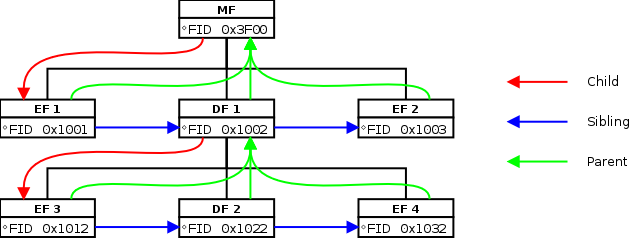
\includegraphics[scale=0.4]{fs_table.png}
\caption{Pembagian file system}
\label{fig-file-relation}
\end{figure}

Sebagaimana dijelaskan pada \nameref{block-concept}, setiap unit data di dalam {\em file system} dialamati menggunakan nomor {\em block} yang berukuran 2 byte. 

\subsection{Bagian-bagian file system}
\label{fs-partitioning}

Oleh {\em file system}, ruang memory virtual yang disediakan {\em HAL Memory} dibagi menjadi tiga bagian besar, yaitu :
\begin{itemize}
\item Block Allocation Table (BAT)
\item File Table
\item File Body
\end{itemize}

Susunan ketiga bagian ini pada memory ditampilkan pada Gambar \ref{fig-fs-partition}.

\begin{figure}[h]
\centering
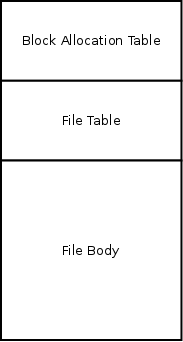
\includegraphics[scale=0.5]{fs_general.png}
\caption{Pembagian file system}
\label{fig-fs-partition}
\end{figure}

\subsubsection{Block Allocation Table}

{\em Block Allocation Table} (BAT) berfungsi menyimpan informasi mengenai {\em block} mana saja yang telah digunakan dan {\em block} mana yang belum. Setiap bit dari {\em block allocation table} merujuk pada sebuah {\em block}, dimana untuk {\em block} yang telah digunakan ditandai dengan nilai 1, sedangkan {\em block} yang tidak digunakan ditandai dengan nilai 0. Gambar \ref{fig-bat} menampilkan contoh penggunaan {\em block allocation table} untuk menyimpan informasi penggunaan {\em block} pada {\em file system}. {\em Block} yang dirujuk oleh sebuah bit pada {\em block allocation table} dapat dihitung menggunakan rumus :
$$
block\_address=byte\_number\cdot8+bit\_number
$$

\begin{figure}[t]
\centering
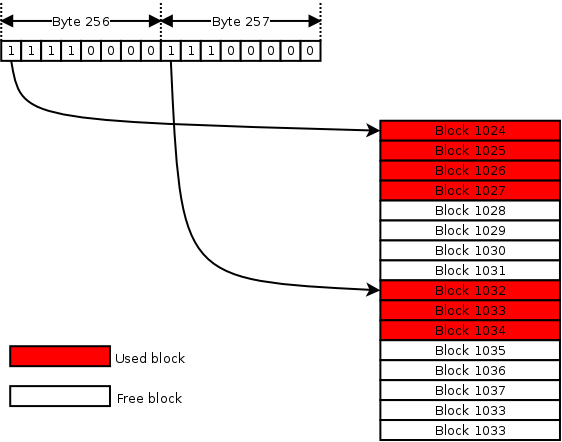
\includegraphics[scale=0.4]{fs_bat.png}
\caption{Contoh penggunaan block allocation table}
\label{fig-bat}
\end{figure}

Total ruang memory yang digunakan oleh {\em Block Allocation Table} dalam byte dapat dihitung mengggunakan rumus :
$$
BAT\_size=(memory\_size/block\_size)/8
$$

Sebagai contoh, untuk sistem dengan ruang memory penyimpanan sebesar 128 kB dan ukuran {\em block} {\tt 4} byte, maka besar ruang yang dibutuhkan untuk {\em block allocation table} adalah $128kB/4B=32kbit=4kB$.

Perlu diingat bahwa {\em block allocation table} akan mengurangi ruang memory virtual yang dapat digunakan untuk menyimpan informasi aktual. Tingkat kerugian penggunaan ruang memory yang diakibatkan oleh {\em block allocation memory} dapat dihitung sebagai perbandingan bagian memory yang digunakan untuk {\em block allocation table} terhadap seluruh ruang memory yang disediakan.
$$
kerugian=BAT\_size/memory\_size=8/block\_size
$$

Terlihat bahwa kerugian akibat {\em block allocation table} berbanding terbalik dengan ukuran {\em block}. Karenanya, hal ini juga harus menjadi perhatian saat menentukan ukuran {\em block}.

\subsubsection{File Table}
\label{file-table}

{\em File Table} berfungsi menyimpan informasi mengenai struktur {\em file system} sebagai hubungan dari sejumlah file yang berawal dari sebuah MF (lihat \nameref{fs-structure}). Informasi-informasi dasar dari setiap file disimpan dalam sebuah struktur data yang dinamakan {\em file header}. Sejumlah {\em file header} yang saling terhubung inilah yang kemudian disimpan di dalam file table untuk membentuk struktur {\em file system}.

\begin{figure}[h]
\centering
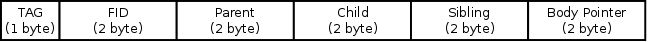
\includegraphics[scale=0.4]{fs_header.png}
\caption{Struktur data file header}
\label{fig-header-field}
\end{figure}

\begin{figure}
\centering
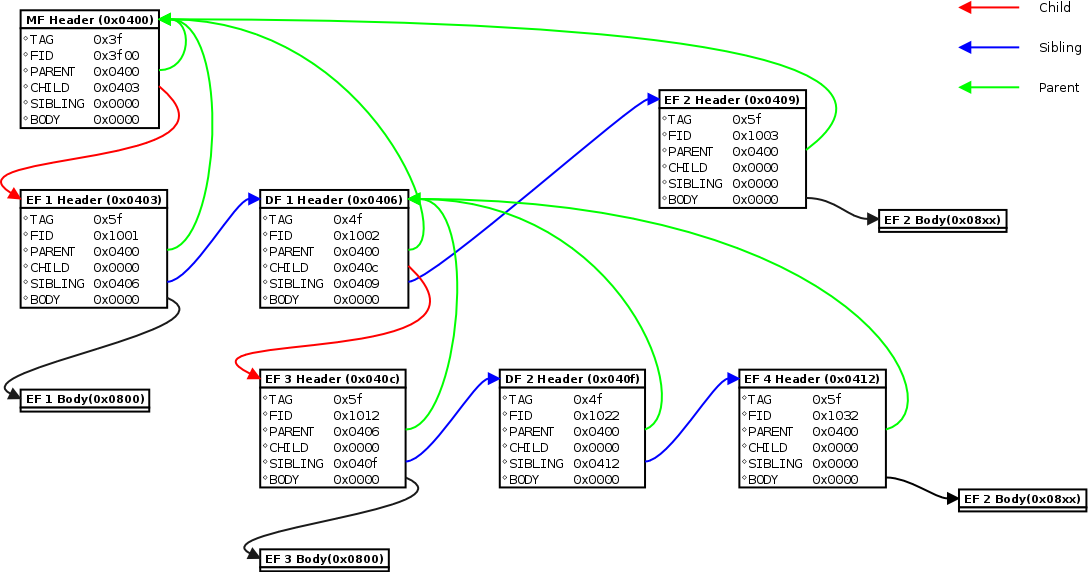
\includegraphics[angle=90,scale=0.4]{fs_table_complete.png}
\caption{Struktur file header lengkap dari contoh sebuah file system (Gambar \ref{fig-fs-example}}
\label{fig-header-complete}
\end{figure}

\begin{figure}
\centering
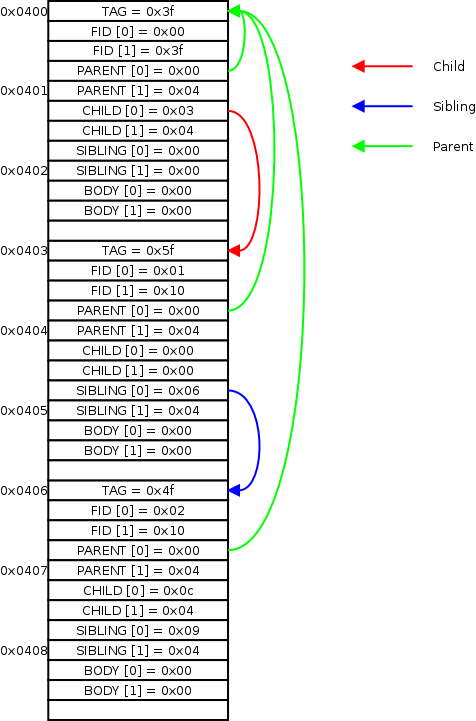
\includegraphics[scale=0.4]{fs_table_memory.png}
\caption{Susunan file header dari contoh sebuah file system (Gambar \ref{fig-fs-example}}
\label{fig-header-memory}
\end{figure}

Gambar \ref{fig-header-field} menampilkan struktur akhir dari sebuah {\em file header}. Kemudian Gambar \ref{fig-header-complete} menampilkan contoh struktur {\em file header} lengkap dari {\em file system} yang ditunjukkan pada Gambar \ref{fig-fs-example}. Susunan struktur {\em file header} ini pada {\em virtual memory} kemudian ditampilkan pada Gambar \ref{fig-header-memory}.


\begin{description}[leftmargin=2.5cm,style=sameline]

\item[Tag] Merupakan indikasi mengenai jenis sebuah file. (Lihat bagian \nameref{file-attribute}.)

\begin{table}[htbp]
  \centering
  \begin{tabular}{|c|c|}
    \hline
    File Type & Tag\\[5pt]
    \hline
    MF        & 0x3F\\
    DF        & 0x4F\\
    EF        & 0x5F\\
    \hline
  \end{tabular}
  \caption{File Tag}
  \label{"tbl-file-tag}
\end{table}


\item[FID] Merupakan pengenal dari sebuah file dalam \textsl{smart card}. (Lihat bagian \nameref{file-attribute}.)

\item[Parent] Merupakan pointer yang menyimpan alamat dari file {\em parent}. (Lihat \nameref{fs-structure}.)

\item[Child] Merupakan pointer yang menyimpan alamat dari file {\em child} pertama. (Lihat \nameref{fs-structure}.)

\item[Sibling] Merupakan pointer yang menyimpan alamat dari file {\em sibling} berikutnya. (Lihat \nameref{fs-structure}.)

\item[File Body] Merupakan pointer yang menyimpan alamat dari bagian file body dari file. (Mengenai file body ini akan dijelaskan lebih rinci pada bagian \nameref{file-body}.)

\end{description}


\subsubsection{File Body}
\label{file-body}

Bagian ini diperuntukkan bagi isi dari file yang sebenarnya. Isi file ini akan tergabung dalam sebuah struktur {\em file body} yang terdiri dari {\em File Body Header} dan {\em File Body Data}. {\em File Body Header} mengandung deskripsi dari isi {\em File Body Data} dan beberapa atribut lainnya yang terkait dengan File. Data aktual dari file sendiri disimpan pada {\em File Body Data}. Gambar \ref{fig-body} menampilkan struktur dari {\em File Body}

\begin{figure}[h]
  \centering
  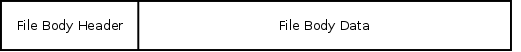
\includegraphics[width=\linewidth]{fs_file_body.png} 
  \caption{Struktur File Body}
  \label{fig-body}
\end{figure}


Gambar \ref{fig-body-header} menampilkan struktur data dari {\em File Body Header}.

\begin{figure}[h]
\centering
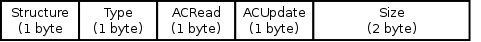
\includegraphics[scale=0.4]{fs_body_header.png}
\caption{Pembagian file system}
\label{fig-body-header}
\end{figure}


\begin{description}[leftmargin=3cm,style=sameline]

\item[Structure] Menunjukkan struktur file yang digunakan. Sesuai dengan standard ISO 7816-4, maka struktur file yang didukung terdiri dari : Transparent, Record, dan Cyclic. Setiap struktur file ini akan diberi tag sendiri untuk membedakannya dari struktur file lain sebagaimana ditampilkan pada Tabel \ref{table-file-structure-tag}.

\item[Type] Menunjukkan tipe file. Sesuai dengan standard ISO 7816-4, sebuah file dapat berupa working file ataupun internal file. working file dapat dibaca oleh aplikasi dan sistem operasi, sedangkan internal file hanya dapat dibaca oleh sistem operasi. Sebagaimana File Structure, setiap File Type ini diberi Tag untuk membedakannya dari File Type lain yang ditunjukkan pada Tabel \ref{table-file-type}.

\item[Access cond.] Menunjukkan tingkat keamanan yang harus dicapai sebelum melakukan operasi terhadap file, masing-masing AC read untuk operasi baca dan ACUpdate untuk operasi tulis. Nilai-nilai ini akan diverifikasi oleh State Manager.

\item[Size] Menunjukkan ukuran data file dalam byte. 

\end{description}




\section{Function}

\begin{figure}[h]
\centering
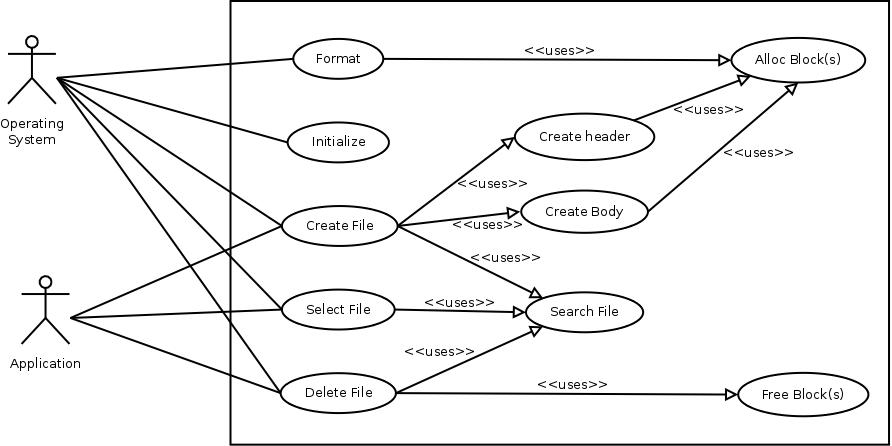
\includegraphics[scale=0.3]{fs_usecase.png}
\caption{Pembagian file system}
\label{fig-usecase}
\end{figure}

Fungsi-fungsi yang terdapat pada {\em File System} dan hubungannya dapat dilihat melalui use case diagram pada Gambar \ref{fig-usecase}. Dari usecase diagram tersebut terlihat fungsi-fungsi yang ada pada {\em file system} sebagai berikut :

\begin{description}[labelindent=1cm,leftmargin=4.2cm,style=sameline]

\item[Format] Format the filesystem.
\item[Initialize] Initialize the filesystem.
\item[Search File] Search for a file
\item[Select File] Select a file
\item[Create File] Create a new file
\item[Create Header] Create a new file header
\item[Create Body] Create a new file body
\item[Delete File] Delete a file 
\item[Access Binary] Access a transparent file
\item[Access Record] Operate on a record file
\item[Alloc Block(s)] Alloc block(s) of memory
\item[Free Block(s)] Free block(s) of memory

\end{description}


\subsection{Format}

Fungsi {\em Format} akan mempersiapkan memory untuk penggunaan pertama file system. Fungsi ini hanya sekali dipanggil oleh system operasi ketika finalisasi \textsl{smart card}. Fungsi ini akan diimplementasikan sebagai FSFormat() dan tidak menerima argumen apapun. Hasil keluaran dari fungsi adalah keterangan apakah fungsi berhasil atau mengalami kesalahan (error).

\begin{table}[htbp]
  \centering
  \begin{tabular}{p{2cm}p{8cm}}
    \hline\\
    {\bf Name} & FSFormat\\
    \hline\\
    {\bf Input}  & None\\
    \hline\\
    {\bf Output} & 
    \begin{itemize}[noitemsep,topsep=0pt,parsep=0pt,partopsep=0pt]
    \item Status
    \end{itemize}
    \\
    \hline
  \end{tabular}
  \caption{Prototype Fungsi Format}
  \label{tbl-format}
\end{table}

%% \begin{description}[labelindent=1cm,leftmargin=2cm,style=sameline]
%% \item[Name] FSFormat()
%% \item[Input] Tidak ada
%% \item[Output] Status
%% \end{description}

\begin{figure}[h]
\centering
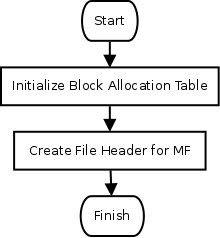
\includegraphics[scale=0.4]{fs_format.png}
\caption{Algoritma fungsi format}
\label{fig-format}
\end{figure}

Gambar \ref{fig-format} menampilkan prosedur yang dijalankan oleh fungsi {\em Format}. Fungsi {\em Format} akan mempersiapkan memory dengan menghapus seluruh isi memory dan membagi memory menjadi bagian-bagian sebagaimana dijelaskan pada Bagian \nameref{fs-partitioning}. Setelah itu fungsi akan membuat file root (MF) di alamat pertama pada {\em File Table}. 


\subsection{Initialize}

Fungsi {\em Initialize} akan mempersiapkan memory untuk dapat dipergunakan. Fungsi ini dipanggil oleh sistem operasi setiap kali \textsl{memory card} diberi daya dan memasuki tahap initialisasi. Fungsi ini akan diimplementasikan sebagai FSInitialize() dan tidak menerima argumen apapun. Hasil keluaran dari fungsi adalah status apakah fungsi berhasil atau mengalami kesalahan (error).

\begin{table}[htbp]
  \centering
  \begin{tabular}{p{2cm}p{8cm}}
    \hline\\
    {\bf Name} & FSInitialize\\
    \hline\\
    {\bf Input}  & None\\
    \hline\\
    {\bf Output} & 
    \begin{itemize}[noitemsep,topsep=0pt,parsep=0pt,partopsep=0pt]
    \item Status
    \end{itemize}
    \\
    \hline
  \end{tabular}
  \caption{Prototype Fungsi Initialize}
  \label{tbl-initialize}
\end{table}

%% \begin{description}[labelindent=1cm,leftmargin=2cm,style=sameline]
%% \item[Name] FSInitialize
%% \item[Input] Tidak ada
%% \item[Output] Status
%% \end{description}

Gambar \ref{fig-initialize} menampilkan prosedur yang dijalankan oleh fungsi {\em Initialize}.

\begin{figure}[h]
\centering
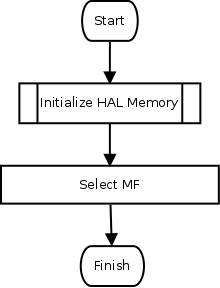
\includegraphics[scale=0.3]{fs_initialize.png}
\caption{Algoritma fungsi Initialize}
\label{fig-initialize}
\end{figure}


\subsection{Create File}

Fungsi {\em Create File} akan menciptakan sebuah file baru pada struktur {\em file system}. Fungsi ini dapat dipanggil oleh sistem operasi maupun aplikasi. Fungsi ini akan diimplementasikan sebagai FSCreateFile().

\begin{table}[htbp]
  \centering
  \begin{tabular}{p{2cm} p{8cm}}
    \hline\\
    {\bf Name} & FSCreateFile\\
    \hline\\
    {\bf Input} & 
    \begin{itemize}[noitemsep,topsep=0pt,parsep=0pt,partopsep=0pt]
    \item File descriptor
    \end{itemize}
    \\
    \hline\\
    {\bf Output} & 
    \begin{itemize}[noitemsep,topsep=0pt,parsep=0pt,partopsep=0pt]
    \item Status
    \end{itemize}
    \\
    \hline
  \end{tabular}
  \caption{Prototype Fungsi Create File}
  \label{tbl-create-file}
\end{table}

%% \begin{description}[labelindent=1cm,leftmargin=2cm,style=sameline]
%% \item[Name] FSCreateFile
%% \item[Input] \mbox{}\\[-1.5\baselineskip]
%%   \begin{itemize}
%%   \item File descriptor
%%   \end{itemize}
%% \item[Output]\mbox{}\\[-1.5\baselineskip]
%%   \begin{itemize}
%%   \item Block address of header of file created
%%   \item Keterangan
%%   \end{itemize}
%% \end{description}

Gambar \ref{fig-create-file} menampilkan prosedur yang dijalankan oleh fungsi Create File. File baru hanya dapat dibuat apabila file yang sedang terpilih adalah sebuah DF, dimana file baru ini akan diletakkan dibawahnya (sebagai anak) pada struktur file system. Selain itu tidak boleh ada file lainnya dalam jangkauan parent yang memiliki FID yang sama dengan file baru agar tidak menimbulkan ambiguitas.

\begin{figure}
\centering
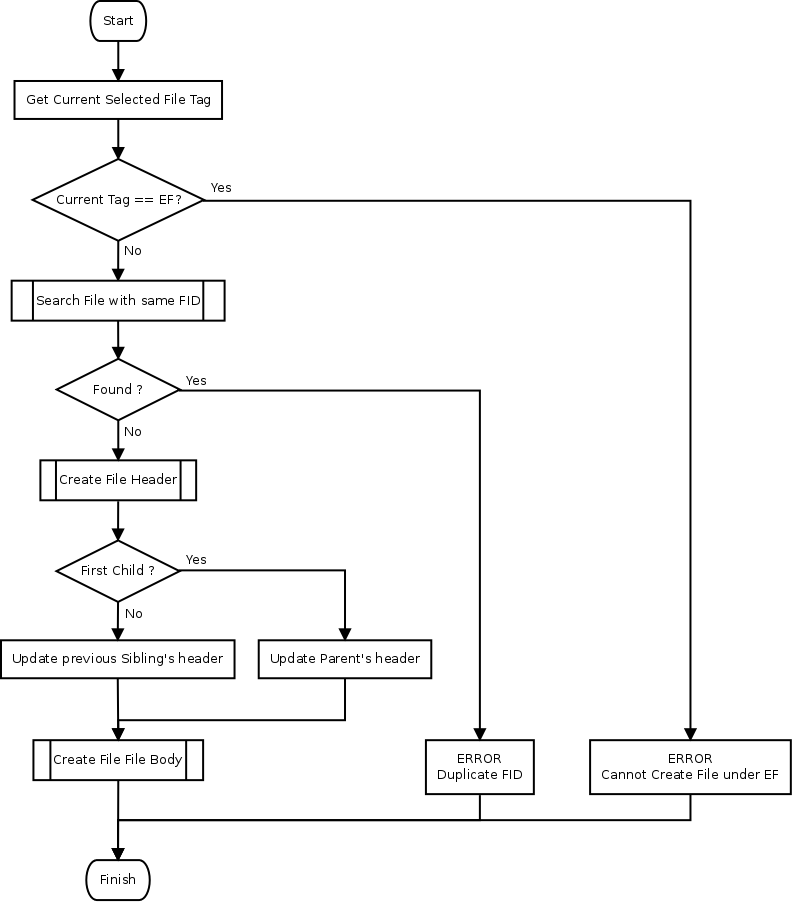
\includegraphics[width=\linewidth]{fs_create_file.png}
\caption{Algoritma fungsi Create File}
\label{fig-create-file}
\end{figure}

Apabila semua syarat telah terpenuhi, Sebuah file baru akan dibuat dengan menghasilkan sebuah file header dengan memanggil fungsi {\em Create Header}. Apabila fungsi {\em Create Header} berhasil membuat file header baru, maka prosedur dilanjutkan dengan memperbaharui file header dari {\em parent} atau {\em sibling}, tergantung apakah file baru tersebut merupakan {\em child} pertama atau tidak dari {\em parent} file. Pada kasus {\em child} pertama, maka yang perlu diperbaharui adalah pointer {\em child} dari {\em parent} file (lihat Gambar \ref{fig-create-file-example-1}). Sementara pada kasus {\em child} kedua dan seterusnya, maka yang diperbaharui adalah pointer {\em sibling} dari file {\em sibling} sebelumnya (lihat Gambar \ref{fig-create-file-example-2}).

\begin{figure}
\centering
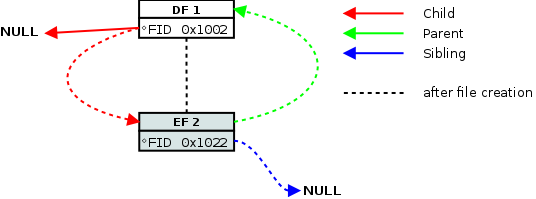
\includegraphics[scale=0.4]{fs_create_file_example_1.png}
\caption{Contoh fungsi Create File (kasus {\em child} pertama)}
\label{fig-create-file-example-1}
\end{figure}

\begin{figure}
\centering
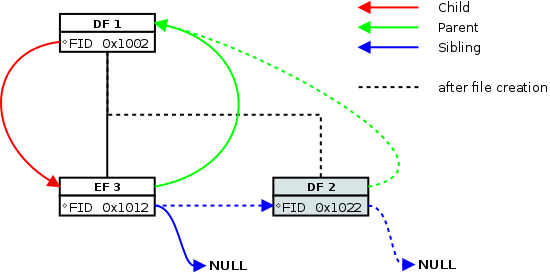
\includegraphics[scale=0.3]{fs_create_file_example_2.png}
\caption{Contoh fungsi Create File (kasus {\em child} kedua)}
\label{fig-create-file-example-2}
\end{figure}

Setelah file header dari file parent/sibling diperbaharui, fungsi kemudian akan membuat sebuah file body (dengan memanggil fungsi Create Body) dengan atribut yang sesuai dengan file descriptor yang diberikan pada masukan fungsi. Apabila file body berhasil dibuat, maka file header yang telah dibuat sebelumnya akan diperbaharui dengan memasukkan alamat file body. Namun apabila file body tidak berhasil dibuat, maka file header yang telah dibuat sebelumnya harus dihapus dengan memanggil fungsi Delete File.


\subsection{Delete File}

Fungsi {\em Delete File} akan menghapus sebuah file dari struktur file system. Fungsi ini dapat dipanggil oleh sistem operasi maupun aplikasi. Fungsi ini akan diimplementasikan sebagai FSDeleteFile().

\begin{table}[hp]
  \centering
  \begin{tabular}{p{2cm} p{8cm}}
    \hline\\
    {\bf Name} & FSDeleteFile\\
    \hline\\
    {\bf Input} & 
    \begin{itemize}[noitemsep,topsep=0pt,parsep=0pt,partopsep=0pt]
    \item FID
    \end{itemize}
    \\
    \hline\\
    {\bf Output} & 
    \begin{itemize}[noitemsep,topsep=0pt,parsep=0pt,partopsep=0pt]
    \item Status
    \end{itemize}
    \\
    \hline
  \end{tabular}
  \caption{Prototype Fungsi Delete File}
  \label{tbl-delete-file}
\end{table}

%% \begin{description}
%% \item[name] FSDeleteFile
%% \item[input] 
%%   \begin{itemize}
%%   \item FID
%%   \end{itemize}
%% \item[output]
%%   \begin{itemize}
%%   \item Keterangan
%%   \end{itemize}
%% \end{description}

Gambar \ref{fig-delete-file} menampilkan prosedur yang dijalankan oleh fungsi Delete File. Pertama, file yang akan dihapus dicari dengan memanggil fungsi Search File. Setelah ditemukan, file header dari parent / sibling diperbarui sehingga tidak lagi menunjuk pada file yang akan dihapus. Gambar \ref{fig-delete-file-example-1}-\ref{fig-delete-file-example-3} menampilkan beberapa contoh kasus penghapusan file. 

\begin{figure}
\centering
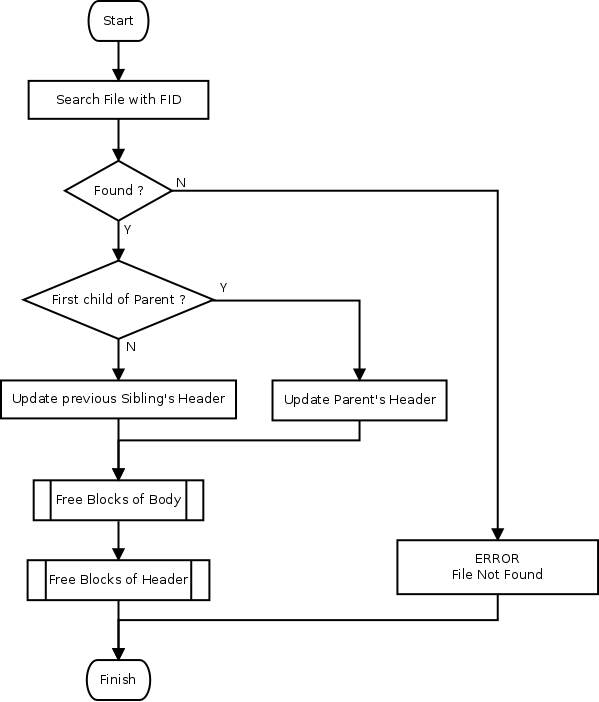
\includegraphics[scale=0.4]{fs_delete_file.png}
\caption{Algoritma fungsi Delete File}
\label{fig-delete-file}
\end{figure}

Pada kasus pertama (Gambar \ref{fig-delete-file-example-1}), file yang dihapus (EF3) merupakan anak pertama dari file parent (DF1). Untuk itu perlu dilakukan pembaruan pada pointer child dari file parent header sehingga menunjuk pada file sibling dari file yang akan dihapus (DF2). 

\begin{figure}
\centering
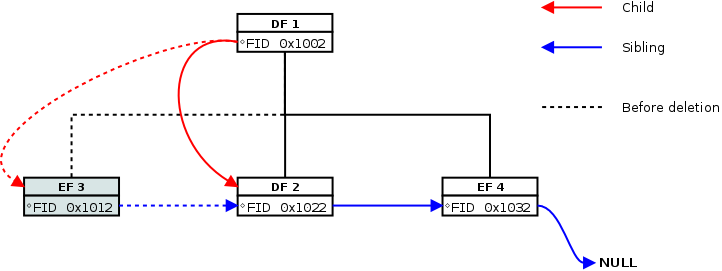
\includegraphics[width=\linewidth]{fs_delete_file_example_1.png}
\caption{Contoh penghapusan file (kasus anak pertama)}
\label{fig-delete-file-example-1}
\end{figure}

Pada kasus kedua (Gambar \ref{fig-delete-file-example-2}), file yang dihapus (DF2) bukan merupakan anak pertama dan bukan pula yang terakhir dari file parent (DF1). Untuk itu perlu dilakukan pembaruan pada pointer sibling dari file sibling sebelumnya (EF3) sehingga menunjuk pada file sibling dari file yang akan dihapus (EF4). 

\begin{figure}
\centering
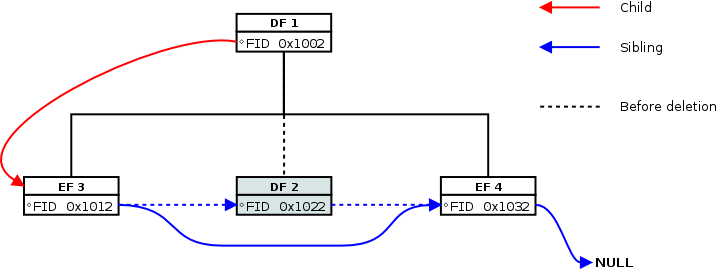
\includegraphics[width=\linewidth]{fs_delete_file_example_2.png}
\caption{Contoh penghapusan file (kasus bukan anak pertama/terakhir)}
\label{fig-delete-file-example-2}
\end{figure}

Pada kasus ketiga (Gambar \ref{fig-delete-file-example-3}), file yang dihapus (EF4) merupakan anak yang terakhir dari file parent (DF1). Untuk itu perlu dilakukan pembaruan pada pointer sibling dari file sibling sebelumnya (DF2). Karena EF4 tidak memiliki sibling berikutnya, maka pointer sibling dari file sibling DF2 akan menunjuk ke NULL.

\begin{figure}
\centering
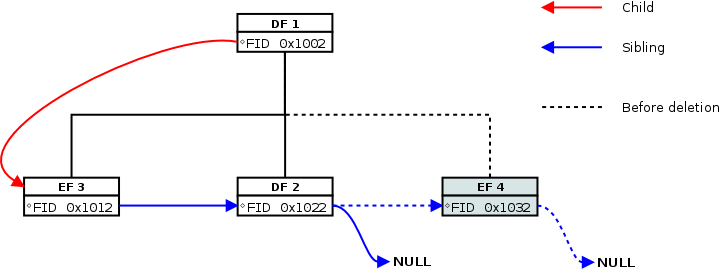
\includegraphics[width=\linewidth]{fs_delete_file_example_3.png}
\caption{Contoh penghapusan file (kasus anak terakhir)}
\label{fig-delete-file-example-3}
\end{figure}


\subsection{Select File}

Fungsi Select File akan mengganti state file yang sedang terpilih dari smart card menjadi file dengan FID yang diberikan. Fungsi ini akan diimplementasi oleh FSSelectFile(). 

\begin{table}[h]
  \centering
  \begin{tabular}{p{2cm} p{8cm}}
    \hline\\
    {\bf Name} & FSSelectFile\\
    \hline\\
    {\bf Input} & 
    \begin{itemize}[noitemsep,topsep=0pt,parsep=0pt,partopsep=0pt]
    \item FID
    \end{itemize}
    \\
    \hline\\
    {\bf Output} & 
    \begin{itemize}[noitemsep,topsep=0pt,parsep=0pt,partopsep=0pt]
    \item Status
    \end{itemize}
    \\
    \hline
  \end{tabular}
  \caption{Prototype Fungsi Select File}
  \label{tbl-select-file}
\end{table}



%% \begin{description}
%% \item[name] FSSelectFile
%% \item[input] 
%%   \begin{itemize}
%%   \item FID of file to select
%%   \end{itemize}
%% \item[output]
%%   \begin{itemize}
%%   \item Status
%%   \end{itemize}
%% \end{description}

Gambar \ref{fig-select-file} menampilkan prosedur yang dijalankan oleh fungsi Select File. Pertama, file yang akan dipilih dicari dengan memanggil fungsi Search File. Apabila file ditemukan, maka state saat ini akan diubah sehingga menunjuk pada file yang dipilih. Sebaliknya apabila tidak ditemukan maka akan mengembalikan nilai kesalahan {\em File Not Found}.

\begin{figure}
\centering
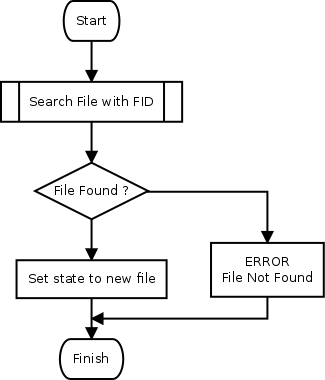
\includegraphics[scale=0.3]{fs_select_file.png}
\caption{Algoritma fungsi Select File}
\label{fig-select-file}
\end{figure}


\subsection{Access Binary}

Fungsi {\em Access Binary} dipanggil oleh sistem operasi atau aplikasi untuk mengakses file EF bertipe transparent. Sebelum memanggil fungsi Access Binary maka sistem operasi atau aplikasi harus memilih file yang akan diakses menggunakan fungsi {\em File Select}. 

\begin{table}[hp]
  \centering
  \begin{tabular}{p{2cm} p{8cm}}
    \hline\\
    {\bf Name} & FSAccessBinary\\
    \hline\\
    {\bf Input} & 
    \begin{itemize}[noitemsep,topsep=0pt,parsep=0pt,partopsep=0pt]
    \item Operation (Read or Update)
    \item Offset (in bytes)
    \item Lenght of data to read/update
    \item Data to update
    \end{itemize}
    \\
    \hline\\
    {\bf Output} & 
    \begin{itemize}[noitemsep,topsep=0pt,parsep=0pt,partopsep=0pt]
    \item Data readed
    \item Status
    \end{itemize}
    \\
    \hline
  \end{tabular}
  \caption{Prototype Fungsi Access Binary}
  \label{tbl-access-binary}
\end{table}

Terdapat dua jenis operasi yang dapat dilakukan, yaitu Read dan Update. Operasi Read akan membaca data dari file yang sedang dipilih dan mengembalikan ke fungsi pemanggil. Sementara Operasi Update akan mengubah data pada file dengan data yang berasal dari fungsi pemanggil. Fungsi ini akan diimplementasikan oleh FSAccessBinary().

\begin{figure}
\centering
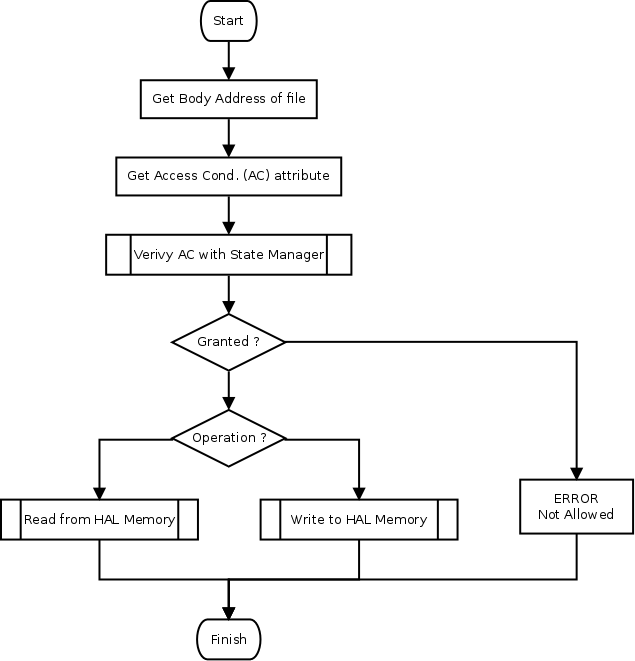
\includegraphics[scale=0.3]{fs_access_binary.png}
\caption{Algoritma fungsi Access Binary}
\label{fig-access-binary}
\end{figure}

Gambar \ref{fig-access-binary} menampilkan prosedur yang dilakukan fungsi access binary. Pertama, fungsi akan mengambil alamat body dari file yang disimpan pada file header. Lalu dari file body tersebut fungsi akan mengambil {\em access condition} yang diperlukan untuk operasi dan diverifikasi ke {\em state manager}. Apabila {\em state manager} menyetujui akses, fungsi akan dilanjutkan dengan melakukan operasi yang diminta (baca/tulis). Sebaliknya apabila {\em state manager} tidak menyetujui, fungsi akan mengembalikan status kesalahan {\em Operation Not Allowed}.

%% \begin{description}
%% \item[name] FSAccessBinary
%% \item[input] 
%%   \begin{itemize}
%%   \item Operasi yang akan dilakukan
%%   \item Offset dari data yang akan diakses
%%   \item Length dari data yang akan diakses
%%   \item data yang akan ditulis apabila operasi Update
%%   \end{itemize}
%% \item[output]
%%   \begin{itemize}
%%   \item data hasil pembacaan apabila operasi Read
%%   \item Status
%%   \end{itemize}
%% \end{description}


\subsection{Access Record}

Fungsi {\em Access Record} dipanggil oleh sistem operasi atau aplikasi untuk mengakses file EF bertipe Record. Sebelum memanggil fungsi {\em Access Record} maka sistem operasi atau aplikasi harus memilih file yang akan diakses menggunakan fungsi {\em File Select}.

\begin{table}[h]
  \centering
  \begin{tabular}{p{2cm} p{8cm}}
    \hline\\
    {\bf Name} & FSAccessRecord\\
    \hline\\
    {\bf Input} & 
    \begin{itemize}[noitemsep,topsep=0pt,parsep=0pt,partopsep=0pt]
    \item Operation (Read/Update/Append/Insert/Delete)
    \item Record No. (for all operation except Append Record)
    \item Lenght of record data (for all operation except Delete Record)
    \item Record data (for all operation except Delete Record)
    \end{itemize}
    \\
    \hline\\
    {\bf Output} & 
    \begin{itemize}[noitemsep,topsep=0pt,parsep=0pt,partopsep=0pt]
    \item Data readed (for Read Operation)
    \item Status
    \end{itemize}
    \\
    \hline
  \end{tabular}
  \caption{Prototype Fungsi Access Record}
  \label{tbl-access-record}
\end{table}

Terdapat lima jenis operasi yang dapat dilakukan, yaitu Read, Update, Append Record, Insert Record, dan Delete Record. Operasi Read akan membaca data record dari file yang sedang dipilih dan mengembalikan ke fungsi pemanggil. Operasi Update akan mengubah data record pada file dengan data record yang berasal dari fungsi pemanggil. Operasi Append akan menambahkan sebuah record baru setelah record yang paling akhir. Operasi Insert akan menambahkan sebuah record baru diantara record yang ada. Operasi Delete akan menghapus sebuah record dari file. Fungsi ini akan diimplementasikan oleh FSAccessRecord().


%% \begin{description}
%% \item[name] FSAccessRecord
%% \item[input] 
%%   \begin{itemize}
%%   \item Operasi yang akan dilakukan
%%   \item No Record yang akan diakses
%%   \item Offset dari data yang akan diakses
%%   \item Length dari data yang akan diakses
%%   \item data yang akan ditulis apabila operasi Update
%%   \end{itemize}
%% \item[output]
%%   \begin{itemize}
%%   \item data hasil pembacaan apabila operasi Read
%%   \item Status
%%   \end{itemize}
%% \end{description}




\subsection{Search File}

Fungsi {\em Search File} dipanggil oleh fungsi-fungsi File System lainnya untuk menemukan file dengan FID yang diberikan. Fungsi ini akan diimplementasikan sebagai FSSearchFile, dan akan mengembalikan alamat block dari file header dari file yang dicari apabila ditemukan, atau NULL apabila file tidak ditemukan.

\begin{table}[h]
  \centering
  \begin{tabular}{p{2cm} p{8cm}}
    \hline\\
    {\bf Name} & FSSearchFile\\
    \hline\\
    {\bf Input} & 
    \begin{itemize}[noitemsep,topsep=0pt,parsep=0pt,partopsep=0pt]
    \item FID
    \end{itemize}
    \\
    \hline\\
    {\bf Output} & 
    \begin{itemize}[noitemsep,topsep=0pt,parsep=0pt,partopsep=0pt]
    \item Block address of file header
    \item Status (if Error)
    \end{itemize}
    \\
    \hline
  \end{tabular}
  \caption{Prototype Fungsi Search File}
  \label{tbl-search-file}
\end{table}

%% \begin{description}
%% \item[name] FSSearchFile
%% \item[input] 
%%   \begin{itemize}
%%   \item FID
%%   \end{itemize}
%% \item[output]
%%   \begin{itemize}
%%   \item alamat block file header dari file yang dicari
%%   \item NULL apabila file tidak ditemukan
%%   \end{itemize}
%% \end{description}


\begin{figure}
\centering
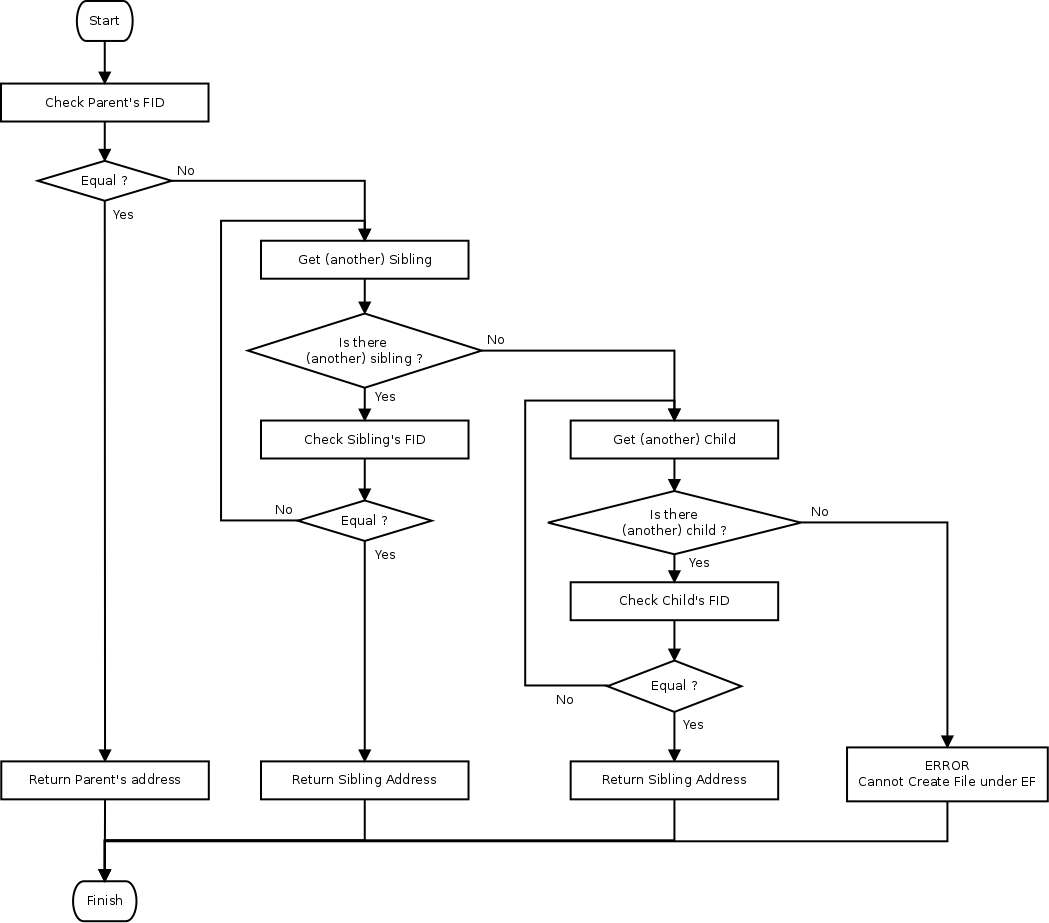
\includegraphics[angle=90,scale=0.3]{fs_search_file.png}
\caption{Algoritma fungsi Search File}
\label{fig-search-file}
\end{figure}

Gambar \ref{fig-search-file} menampilkan prosedur yang dijalankan oleh fungsi Search File. Pencarian akan dilakukan dimulai dari parent file dari file yang sedang terpilih, dilanjutkan dengan memeriksa setiap sibling, dan berikutnya memeriksa seluruh child apabila file yang terpilih adalah sebuah DF. 

\subsection{Create Header}

Fungsi {\em Create Header} dipanggil oleh fungsi Create File untuk menghasilkan sebuah file header baru pada file table berdasarkan file descriptor yang diberikan. Fungsi ini akan diimplementasikan sebagai FSCreateHeader().

\begin{table}[hp]
  \centering
  \begin{tabular}{p{2cm} p{8cm}}
    \hline\\
    {\bf Name} & FSCreateHeader\\
    \hline\\
    {\bf Input} & 
    \begin{itemize}[noitemsep,topsep=0pt,parsep=0pt,partopsep=0pt]
    \item File descriptor
    \end{itemize}
    \\
    \hline\\
    {\bf Output} & 
    \begin{itemize}[noitemsep,topsep=0pt,parsep=0pt,partopsep=0pt]
    \item Block address of header created
    \item Status
    \end{itemize}
    \\
    \hline
  \end{tabular}
  \caption{Prototype Fungsi Create Header}
  \label{tbl-create-header}
\end{table}


%% \begin{description}
%% \item[name] FSCreateHeader
%% \item[input] 
%%   \begin{itemize}
%%   \item File descriptor
%%   \end{itemize}
%% \item[output]
%%   \begin{itemize}
%%   \item alamat block pertama dari header yang dihasilkan
%%   \end{itemize}
%% \end{description}

\begin{figure}
\centering
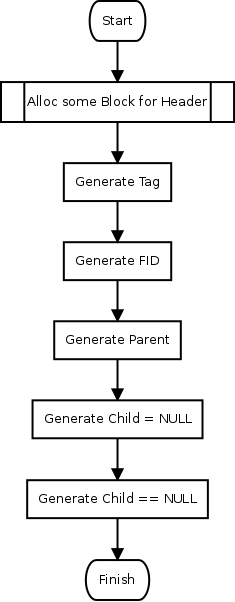
\includegraphics[scale=0.4]{fs_create_header.png}
\caption{Algoritma fungsi Create Header}
\label{fig-create-header}
\end{figure}

Gambar \ref{fig-create-header} menampilkan prosedur yang dijalankan oleh fungsi Create Header. Pertama, fungsi akan mengalokasikan sejumlah block untuk header dengan memanggil fungsi Alloc Block(s). Apabila berhasil, dan sejumlah block telah dialokasikan, maka block tersebut akan diisi dengan struktur data file header sebagaimana yang telah dijelaskan pada bagian \nameref{file-table}. Tag dan FID yang digunakan diambil dari file descriptor, sementara parent merupakan file yang sedang dipilih sekarang yang diperoleh melalui State Manager. Child dan Sibling diisi nilai NULL karena file merupakan sebuah file baru sehingga tidak memiliki child dan sibling. Body pointer dibiarkan barena akan diisi kemudian setelah file body dihasilkan.



\subsection{Alloc Block(s)}

Fungsi {\em Alloc Block(s)} dipanggil oleh fungsi-fungsi lain untuk mengalokasikan sejumlah block untuk digunakan. 

\begin{table}[h]
  \centering
  \begin{tabular}{p{2cm} p{8cm}}
    \hline\\
    {\bf Name} & FSAlloc\\
    \hline\\
    {\bf Input} & 
    \begin{itemize}[noitemsep,topsep=0pt,parsep=0pt,partopsep=0pt]
    \item Begin of Block to search for free blocks
    \item End of Block to search for free blocks
    \item Length of block to alloc
    \end{itemize}
    \\
    \hline\\
    {\bf Output} & 
    \begin{itemize}[noitemsep,topsep=0pt,parsep=0pt,partopsep=0pt]
    \item Address of allocated block
    \item Status (if ERROR)
    \end{itemize}
    \\
    \hline
  \end{tabular}
  \caption{Prototype Fungsi Alloc Block(s)}
  \label{tbl-alloc}
\end{table}


%% \begin{description}
%% \item[name] FSAlloc
%% \item[input] 
%%   \begin{itemize}
%%   \item Begin Block to search for free block
%%   \item End Block to search for free block
%%   \item length of block to allocated
%%   \end{itemize}
%% \item[output]
%%   \begin{itemize}
%%   \item alamat awal block yang telah dialokasikan apabila berhasil
%%   \item NULL apabila tidak menemukan cukup free block
%%   \end{itemize}
%% \end{description}

\begin{figure}
\centering
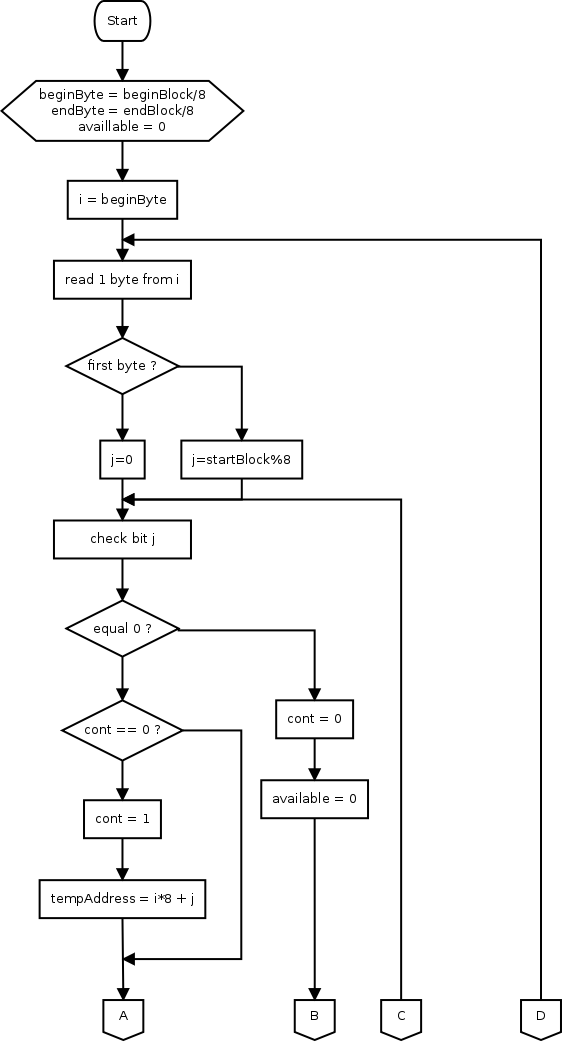
\includegraphics[scale=0.4]{fs_alloc_1.png}
\caption{Algoritma fungsi Alloc Block(s)}
\label{fig-alloc-1}
\end{figure}

\begin{figure}
\centering
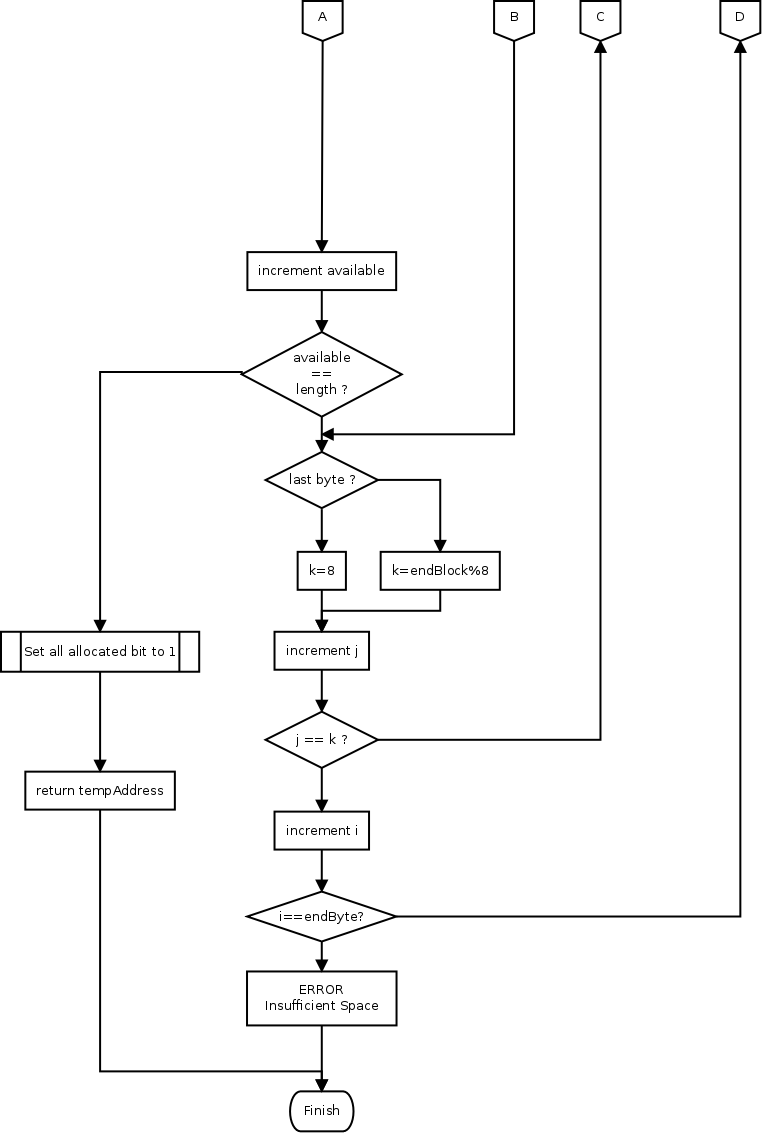
\includegraphics[scale=0.4]{fs_alloc_2.png}
\caption{Algoritma fungsi Alloc Block(s)}
\label{fig-alloc-2}
\end{figure}

Gambar \ref{fig-alloc-1} menampilkan algoritma yang digunakan oleh fungsi Alloc Block(s). Untuk memudahkan memahami algoritma yang digunakan, pada Gambar \ref{fig-alloc-example} menampilkan contoh penggunaan fungsi Alloc Block(s) dengan parameter : 
\begin{itemize}
\item Begin Block = 1026
\item End Block = 1037
\item Length = 3
\end{itemize}


\begin{figure}
\centering
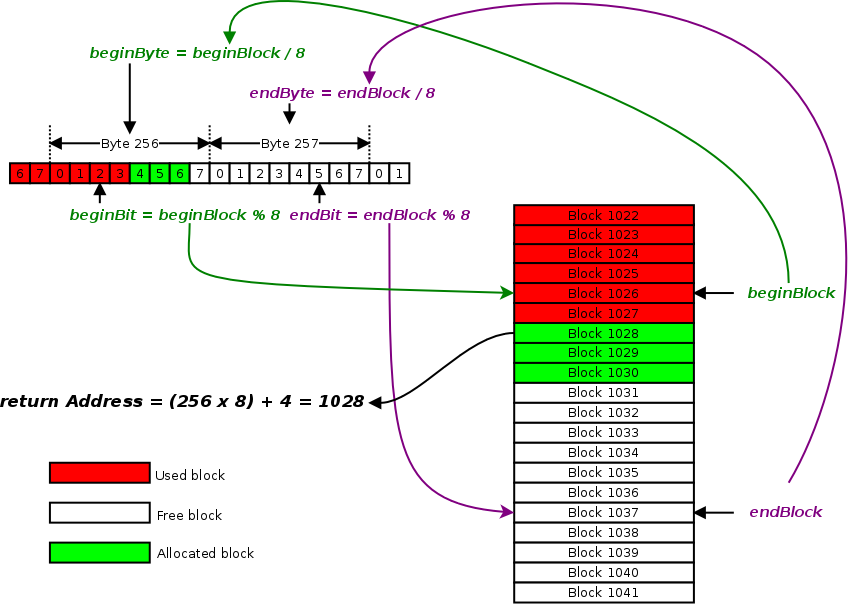
\includegraphics[angle=90,scale=0.5]{fs_alloc_example.png}
\caption{Contoh penggunaan Alloc Block(s)}
\label{fig-alloc-example}
\end{figure}

Block 1026 (begin block) ditunjuk oleh byte ke 256 (=1026/8) dan bit ke 2 (=1026\%8) pada Block Allocation Table (BAT). Sementara Block 1037 (end block) ditunjuk oleh byte ke 257 (=1037/8) dan bit ke 5 (=1037\%8). Karenanya, pencarian block yang bebas dimulai dari byte 256 (begin byte) bit ke-2 (begin bit) hingga byte 257 (end Byte) bit ke-5 (end Bit). 

Pencarian akan menemukan bahwa 2 block pertama telah digunakan (warna merah) dan terdapat sejumlah block bebas (warna putih) yang cukup untuk memenuhi permintaan dimulai dari block 1028, yang ditunjuk oleh byte ke 256 dan bit ke-4 dari BAT. Fungsi Alloc Block(s) kemudian akan menandai ketiga block ini (warna hijau) sebagai block yang telah digunakan pada BAT, dan mengembalikan nilai 1028 sebagai awal block yang dialokasikan ke fungsi pemanggil.


\subsection{Free Block(s)}

Fungsi {\em Free Block(s)} merupakan kebalikan dari fungsi {\em Alloc Block(s)}, dimana sejumlah block yang telah dialokasikan (ditandai dengan nilai 1 pada bit yang bersesuaian di {\em block allocation table}) dibebaskan sehingga dapat dipergunakan kembali nantinya. Fungsi ini utamanya akan dipanggil oleh fungsi {\em Delete File}. Pembebasan dilakukan dengan mengubah nilai bit pada {\em block allocation table} menjadi 0 kembali.

\begin{table}[h]
  \centering
  \begin{tabular}{p{2cm} p{8cm}}
    \hline\\
    {\bf Name} & FSAlloc\\
    \hline\\
    {\bf Input} & 
    \begin{itemize}[noitemsep,topsep=0pt,parsep=0pt,partopsep=0pt]
    \item Begin of block to free
    \item Length of block to free
    \end{itemize}
    \\
    \hline\\
    {\bf Output} & 
    \begin{itemize}[noitemsep,topsep=0pt,parsep=0pt,partopsep=0pt]
    \item Status
    \end{itemize}
    \\
    \hline
  \end{tabular}
  \caption{Prototype Fungsi Free Block(s)}
  \label{tbl-free}
\end{table}



\chapter{Testing}

\chapter{Implementation}

\end{document}
